%==================================================================================================================
%===================================== Présentation de la photocathode ============================================
%==================================================================================================================

\section{Présentation de la photocathode}

\begin{frame}[t]{Présentation de la photocathode}

  \vspace{0.3em}

  \begin{columns}[T,onlytextwidth]

    % ------------------ Colonne gauche ------------------
    \column{0.54\textwidth}

      \begin{pcbanner}{Réactions mises en jeu}
        \footnotesize
        \vspace{0.4em}
        \textbf{\color{pcNavy!70}Anode}\\[0.3em]
        \centerline{\normalsize\ch{H2O -> 2 H+ + 2 e- + 1/2 O2}}\\[0.9em]
        \textbf{\color{pcNavy}Cathode}\\[0.3em]
        \centerline{\normalsize\ch{CO2 + 2 H+ + 2 e- -> CO + H2O}}
      \end{pcbanner}

      \vspace{0.4em}

      \begin{pcbanner}{Principe}
        \begin{itemize}\footnotesize
          \item Deux parties : photovoltaïque + électrochimique
          \item Soleil $\rightarrow$ Séparation des charges (partie PV)
          \item Electrons $\rightarrow$ Réduction du \ch{CO2} (partie électrochimique)
        \end{itemize}
      \end{pcbanner}

    % ------------------ Colonne droite ------------------
    \column{0.55\textwidth}

      \centering

      \hspace*{-0.75cm}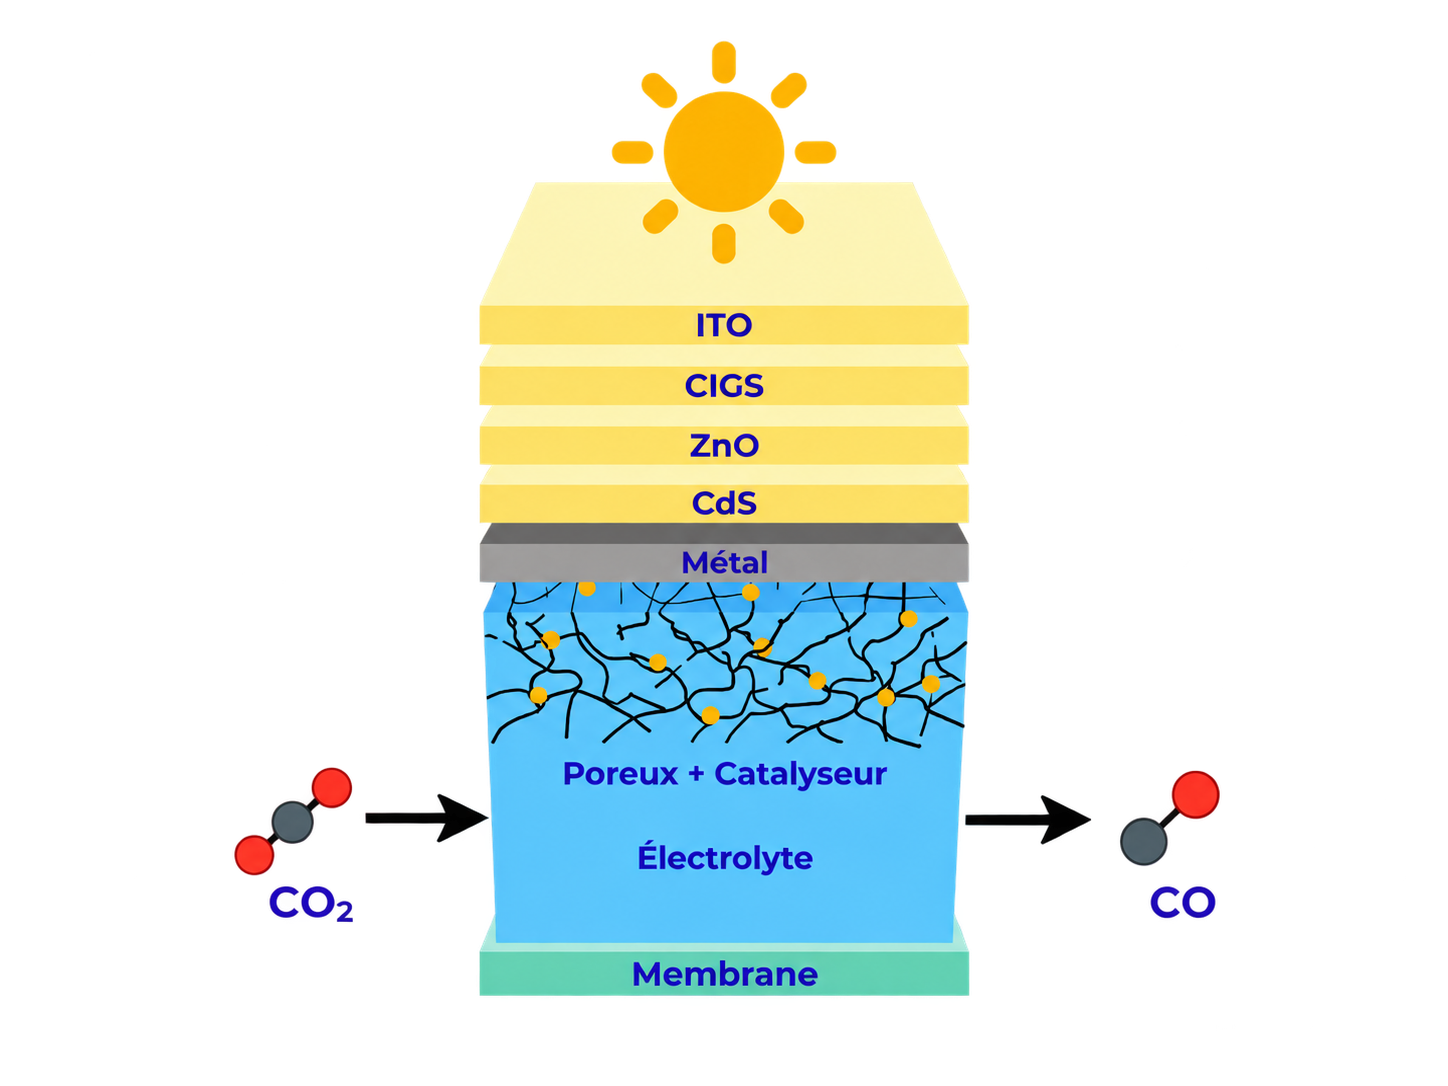
\includegraphics[
        width=1.2\linewidth
      ]{photocathode.png}

  \end{columns}

\end{frame}

%==================================================================================================================
%============================================= Fin Photocathode ===================================================
%==================================================================================================================
